\subsection{Firestorage}

Visto que a desenvolvedora do Flutter e do Firebase é a mesma, esta disponibilizou recursos que facilitam a utilização desta ferramenta pelo Flutter, sendo assim todas as imagens e videos de utilizadores, publicações e comentários são guardadas diretamente da aplicação para o firestorage, assim como o acesso às mesmas é realizado diretamente.

Para permitir este tipo de acesso o Firebase disponibiliza de um configurador de projeto que permite através do terminal configurar a ligação entre o projeto e o servidor do firebase, sendo no final apenas necessário importar a biblioteca do serviço do firebase que se deseja invocar a classe do mesmo sempre que se deseja realizar alguma ação.

Os ficheiros ficam então organizados de acordo com o seu contexto, no caso de utilizadores existe a pasta utilizadores, no caso de tópicos existe a paste tópicos e no caso de comentários existe a pasta comentários. 

Dentro dos utilizadores como cada utilizador apenas contém uma imagem então estas são guardas com o nome do id do utilizador substituindo a imagem anterior se existir. No caso de tópicos e comentários como podem conter várias imagens e videos, então estes são guardados em pastas com ids dos mesmos contendo dentro destas os ficheiros referentes.

\begin{figure}[htb]%
  \centering
  \subfloat[\centering Raiz do firestorage]{{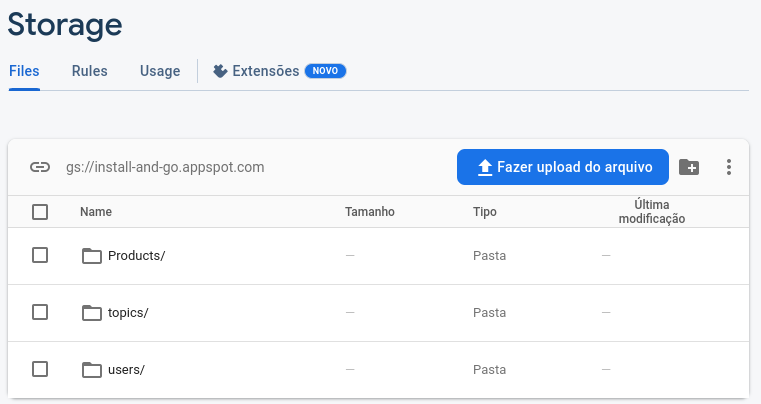
\includegraphics[width=0.7\textwidth]{images/implementacao/frontend/firestorage/all.png} }}%
  \qquad
  \subfloat[\centering Pasta topics do firestorage]{{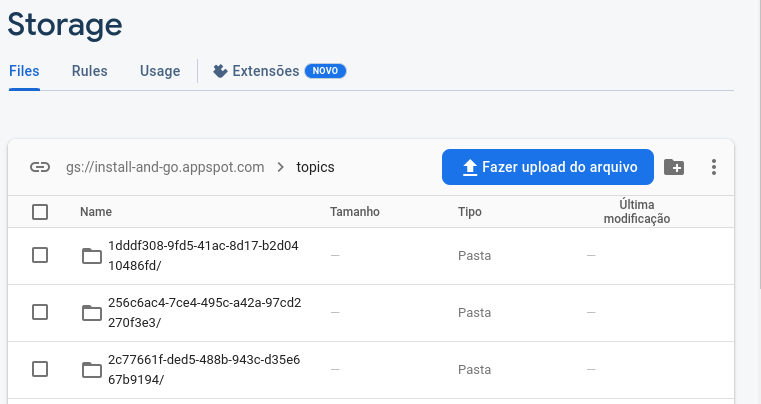
\includegraphics[width=0.7\textwidth]{images/implementacao/frontend/firestorage/topics.png} }}%
  \label{fig:76}%
\end{figure}